\documentclass{beamer}
\usepackage[utf8]{inputenc}
\usepackage{graphicx}
\usepackage{xcolor}
\usepackage{forest}
\usepackage{amsmath}
\usepackage{algorithm}
\usepackage{algpseudocode}
\usepackage[style=authortitle,backend=biber]{biblatex} 
\addbibresource{sample.bib}


\usetheme{Copenhagen}
\useoutertheme{smoothtree} % <<<<<<<<<<<<<<<<<<
\setbeamertemplate{footline}{
  \leavevmode%
  \hbox{%
    \begin{beamercolorbox}[wd=0.33\paperwidth,ht=2.5ex,dp=1ex,center]{author in head/foot}%
      \usebeamerfont{author in head/foot}A. Herrero
    \end{beamercolorbox}%
    \begin{beamercolorbox}[wd=0.34\paperwidth,ht=2.5ex,dp=1ex,center]{title in head/foot}%
      \usebeamerfont{title in head/foot}Random Deletions and Insertions on BST
    \end{beamercolorbox}%
    \begin{beamercolorbox}[wd=0.33\paperwidth,ht=2.5ex,dp=1ex,right]{date in head/foot}%
      \usebeamerfont{date in head/foot}\insertframenumber{} / \inserttotalframenumber\hspace{1em}
    \end{beamercolorbox}%
  }
}

\definecolor{quack}{RGB}{75,0,130}
\usecolortheme[named=quack]{structure}

\begin{document}

\AtBeginSubsection[]
{
  \begin{frame}<beamer>
  \frametitle{Outline}
  \tableofcontents[currentsection,currentsubsection]
  \end{frame}
}

%------------------------------------------------------------
%This block of code defines the information to appear in the
%Title page
% Title page configuration
\title[Random Deletions and Insertions on BST]{
    Project ADS: Random Deletions and Insertions on BST
}

\author[A.Herrero]{
  \begin{minipage}[t]{0.5\textwidth}
    \raggedright
    \small \textit{Author:} \\
    \textbf{Alex Herrero} \\
    \vspace{1cm} % Adjust vertical spacing between author names and professor names
  \end{minipage}%
  \begin{minipage}[t]{0.5\textwidth}
    \raggedleft
    \small \textit{Professors:} \\
    \textbf{Conrado Martínez} \\
    \textbf{Amalia Duch} \\
    \textbf{Salvador Roura} \\
  \end{minipage} \\
  \vspace{1cm} % Adjust space to control the position of the logo
  \begin{center}
    
\includegraphics[scale=0.15]{logo-upc.png}
  \end{center}
}

% Remove navigation symbols
\beamertemplatenavigationsymbolsempty

%End of title page configuration block
%------------------------------------------------------------



%------------------------------------------------------------
\AtBeginSection[ ]
{
    \begin{frame}
        \tableofcontents[currentsection]
    \end{frame}
}
%------------------------------------------------------------

%The next statement creates the title page.
\frame{\titlepage}

\begin{frame}
\frametitle{Acknowledgment}
Special thanks to Conrado Martínez. 
His $\Theta(A(2^{n!}, m\log m))$\footnote{Where $A$ is the Ackermann function. Not the inverse!!} 
wisdom and advice  have been helpful throughout this project.
\end{frame}

%---------------------------------------------------------
%This block of code is for the table of contents after
%the title page
\begin{frame}
    \frametitle{Table of Contents}
    \tableofcontents
\end{frame}
%---------------------------------------------------------

\section{1962: Hibbard}
\begin{frame}{Introduction to BST}
    
\begin{columns}[c]
% Column 1
    \begin{column}{0.5\textwidth}
     \begin{itemize}
         \item He introduced the concept of BST on his paper: ~\fullcite{hibbard1962}.
     \end{itemize}
    \end{column}
% Column 2    
    \begin{column}{0.5\textwidth}
        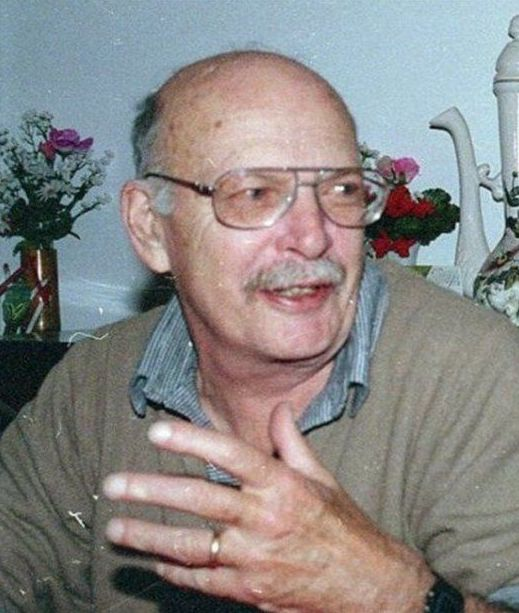
\includegraphics[width=\textwidth]{hibbard.jpg}
        \begin{center}
            Thomas Hibbard (1929-2016)
        \end{center}
    \end{column}
    
\end{columns}
\end{frame}

\begin{frame}
    \begin{itemize}
        \item He introduced not only the concept of binary search trees (BSTs), but also the idea of randomness in BSTs.
            \pause
        \item Well-known concepts and algorithms for every computer scientist.
            \pause
        \item We will take a look to Hibbard's deletion algorithm.
    \end{itemize}
\end{frame}

\begin{frame}{Leaf case}
    \begin{center}
        % Overlay 1: Original Tree
        \only<1>{
            \begin{forest}
                for tree={circle,draw, s sep=10mm}
                [8
                    [3
                        [1]
                        [6
                            [4]
                            [7]
                        ]
                    ]
                    [10
                        [,phantom]
                        [14
                            [13]
                            [,phantom]
                        ]
                    ]
                ]
            \end{forest}
        }

        % Overlay 2: Highlighted leaf
        \only<2>{
            \begin{forest}
                for tree={circle,draw, s sep=10mm}
                [8
                    [3
                        [1]
                        [6
                            [4]
                            [7, color=red]
                        ]
                    ]
                    [10
                        [,phantom]
                        [14
                            [13]
                            [,phantom]
                        ]
                    ]
                ]
            \end{forest}
        }

        % Overlay 3: Leaf removed
        \only<3>{
            \begin{forest}
                for tree={circle,draw, s sep=10mm}
                [8
                    [3
                        [1]
                        [6
                            [4]
                            [,phantom]
                        ]
                    ]
                    [10
                        [,phantom]
                        [14
                            [13]
                            [,phantom]
                        ]
                    ]
                ]
            \end{forest}
        }
    \end{center}
\end{frame}

\begin{frame}{Only one subtree case}
    \begin{center}
        % Overlay 1: Original Tree
        \only<1>{
            \begin{forest}
                for tree={circle,draw, s sep=10mm}
                [8
                    [3
                        [1]
                        [6
                            [4]
                            [7]
                        ]
                    ]
                    [10
                        [,phantom]
                        [14
                            [13]
                            [,phantom]
                        ]
                    ]
                ]
            \end{forest}
        }

        % Overlay 2: Highlighted leaf
        \only<2>{
            \begin{forest}
                for tree={circle,draw, s sep=10mm}
                [8
                    [3
                        [1]
                        [6
                            [4]
                            [7]
                        ]
                    ]
                    [10
                        [,phantom]
                        [14, color=red
                            [13]
                            [,phantom]
                        ]
                    ]
                ]
            \end{forest}
        }

        % Overlay 3: Leaf removed
        \only<3>{
            \begin{forest}
                for tree={circle,draw, s sep=10mm}
                [8
                    [3
                        [1]
                        [6
                            [4]
                            [7]
                        ]
                    ]
                    [10
                        [,phantom]
                        [13]
                    ]
                ]
            \end{forest}
        }
    \end{center}
\end{frame}


\begin{frame}{Two subtree case}
    \begin{center}
        % Overlay 1: Original Tree
        \only<1>{
            \begin{forest}
                for tree={circle,draw, s sep=10mm}
                [8
                    [3
                        [1]
                        [6
                            [4]
                            [7]
                        ]
                    ]
                    [10
                        [,phantom]
                        [14
                            [13]
                            [,phantom]
                        ]
                    ]
                ]
            \end{forest}
        }

        % Overlay 2: Highlighted leaf
        \only<2>{
            \begin{forest}
                for tree={circle,draw, s sep=10mm}
                [8
                    [3, color=red
                        [1]
                        [6
                            [4]
                            [7]
                        ]
                    ]
                    [10
                        [,phantom]
                        [14
                            [13]
                            [,phantom]
                        ]
                    ]
                ]
            \end{forest}
        }

        % Overlay 3: Leaf removed
        \only<3>{
            \begin{forest}
                for tree={circle,draw, s sep=10mm}
                [8
                    [3, color=red
                        [1]
                        [6
                            [4, color=green]
                            [7]
                        ]
                    ]
                    [10
                        [,phantom]
                        [14
                            [13]
                            [,phantom]
                        ]
                    ]
                ]
            \end{forest}
        }
        \only<4>{
            \begin{forest}
                for tree={circle,draw, s sep=10mm}
                [8
                    [4, color=green
                        [1]
                        [6
                            [3, color=red]
                            [7]
                        ]
                    ]
                    [10
                        [,phantom]
                        [14
                            [13]
                            [,phantom]
                        ]
                    ]
                ]
            \end{forest}
        }
        \only<5>{
            \begin{forest}
                for tree={circle,draw, s sep=10mm}
                [8
                    [4, color=green
                        [1]
                        [6
                            [,phantom]
                            [7]
                        ]
                    ]
                    [10
                        [,phantom]
                        [14
                            [13]
                            [,phantom]
                        ]
                    ]
                ]
            \end{forest}
        }
    \end{center}
\end{frame}

\begin{frame}
    \footnotesize
    \begin{algorithmic}
        \Function{delete}{$T$, $x$}
        \If{$T.val < x$}
        \State $T.right \gets$ \Call{delete}{$T.right$, $x$}
        \ElsIf{$T.val > x$}
        \State $T.left \gets$ \Call{delete}{$T.left$, $x$}
        \Else
        \If{$T.right = \text{null}$}
        \State \Return $T.left$
        \Else
        \State $T.val \gets$ \Call{minValue}{$T.right$}
        \State $T.right \gets$ \Call{delete}{$T.right$, $T.val$}
        \EndIf
        \EndIf
        \State \Return $T$
        \EndFunction
    \end{algorithmic}
\end{frame}

\begin{frame}
    Hibbard’s paper was remarkable in that it contained one of the first formal theorems about algorithms:
    \pause
    \begin{block}{Hibbard's Theorem (1962)}
        If $n + 1$ items are inserted into an initially empty binary tree, in random order, and if one of those items (selected at random) is deleted, the probability that the resulting binary tree has a given shape is the same as the probability that this tree shape would be obtained by inserting $n$ items into an initially empty tree, in random order.
    \end{block}
\end{frame}

\section{1975: Knott}

\begin{frame}
    
\begin{columns}[c]
% Column 1
    \begin{column}{0.5\textwidth}
     \begin{itemize}
         \item It was believed for more than a decade that Hibbard's algorithm preserved randomness on BSTs\footnote{In fact this appeared on the first edition of the well-known book \textit{The Art of Computer Programming: Vol 2} by Donald Knuth (1973)}
             \pause
         \item $1975$: \cite{knott1975deletion}
     \end{itemize}
    \end{column}
% Column 2    
    \begin{column}{0.5\textwidth}
        \begin{center}
            \begin{block}{Knott Paradox}
                Although Hibbard’s theorem establishes that n+1 random insertions
                followed by a random deletion produce a tree whose shape has the distribution of n random insertions, it does not follow that a
                subsequent random insertion yields a tree whose shape has the distribution of n+1 random insertions
            \end{block}
        \end{center}
    \end{column}
    
\end{columns}
\end{frame}

\begin{frame}
    We will follow \cite{jonassen1978trivial} for a BST of size $n = 3$
    \pause
    Suppose we have three elements $x < y < z$
\end{frame}

\begin{frame}{All BSTs for $x < y < z$}
    \begin{center}
        \begin{tabular}{cccccc}
            $(x, y, z)$ &
            $(x, z, y)$ &
            $(y, x, z) = (y, z, x)$ &
            $(z, x, y)$ &
            $(z, y, x)$ \\
            \begin{tikzpicture}[level distance=0.6cm,sibling distance=0.6cm]
                \node {x}
                    child[missing]
                    child {node {y}
                        child[missing]
                    child {node {z}}};
            \end{tikzpicture}
                                           &
                                           \begin{tikzpicture}[level distance=0.6cm,sibling distance=0.6cm]
                                               \node {x}
                                                   child[missing]
                                                   child {node {z}
                                                       child {node {y}}
                                                   child[missing]};
                                           \end{tikzpicture}
                                           &
                                           \begin{tikzpicture}[level distance=0.6cm,sibling distance=0.8cm]
                                               \node {y}
                                                   child {node {x}}
                                                   child {node {z}};
                                           \end{tikzpicture}
                                           &
                                           \begin{tikzpicture}[level distance=0.6cm,sibling distance=0.6cm]
                                               \node {z}
                                                   child {node {x}
                                                       child[missing]
                                                   child {node {y}}}
                                                   child[missing];
                                           \end{tikzpicture}
                                           &
                                           \begin{tikzpicture}[level distance=0.6cm,sibling distance=0.6cm]
                                               \node {z}
                                                   child {node {y}
                                                       child {node {x}}
                                                   child[missing]}
                                                   child[missing];
                                           \end{tikzpicture}
                                           \\
            $RR$ & 
            $RL$ &
            $B$ &
            $LR$ &
            $LL$ &
        \end{tabular}
    \end{center}
\end{frame}

\begin{frame}
    \begin{center}
        \begin{tabular}{||c c c c||} 
            \hline
            Permutation& Delete $x$& Delete $y$ & Delete $z$ \\ [0.5ex] 
            \hline\hline
            $(x,y,z)$ & $R$ & $R$ & $R$ \\ 
            \hline
            $(x,z,y)$ & $R$ & $R$ & $R$ \\ 
            \hline
            $(y,z,x) = (y,x,z)$ & $R$ & $L$ & $L$\\ 
            \hline
            $(z,x,y)$ & $L$ & $R$ & $R$\\ 
            \hline
            $(z,y,x)$ & $L$ & $L$ & $L$ \\ 
            \hline
        \end{tabular}
    \end{center}
    \begin{center}
        $\mathbb{P}[L] = \mathbb{P}[R] = \frac{9}{18} = \frac{1}{2}$
    \end{center}
\end{frame}

\begin{frame}
    Now another random insertion $w$ comes to the BST. Then we have four possible cases:
    \begin{itemize}
        \item $w < x < y < z$
        \item $x < w < y < z$
        \item $x < y < w < z$
        \item $x < y < z < w$
    \end{itemize}
    $18$ previous cases and $4$ possibilities for $w$ give us a total of $72$ cases.
\end{frame}

\begin{frame}
    $w < x < y < z$
    \begin{center}
        \begin{tabular}{||c c c c||} 
            \hline
            Permutation& Delete $x$& Delete $y$ & Delete $z$ \\ [0.5ex] 
            \hline\hline
            $(x,y,z)$ & $B$ & $B$ & $B$ \\ 
            \hline
            $(x,z,y)$ & $B$ & $B$ & $B$ \\ 
            \hline
            $(y,z,x) = (y,x,z)$ & $B$ & $LL$ & $LL$\\ 
            \hline
            $(z,x,y)$ & $LL$ & $LL$ & $B$\\ 
            \hline
            $(z,y,x)$ & $LL$ & $LL$ & $LL$ \\ 
            \hline
        \end{tabular}
    \end{center}
\end{frame}

\begin{frame}
    $x < w < y < z$
    \begin{center}
        \begin{tabular}{||c c c c||} 
            \hline
            Permutation& Delete $x$& Delete $y$ & Delete $z$ \\ [0.5ex] 
            \hline\hline
            $(x,y,z)$ & $B$ & $RL$ & $RL$ \\ 
            \hline
            $(x,z,y)$ & $B$ & $RL$ & $RL$ \\ 
            \hline
            $(y,z,x) = (y,x,z)$ & $B$ & $LR$ & $LR$\\ 
            \hline
            $(z,x,y)$ & $LL$ & $LR$ & $RL$\\ 
            \hline
            $(z,y,x)$ & $LL$ & $LR$ & $LR$ \\ 
            \hline
        \end{tabular}
    \end{center}
\end{frame}

\begin{frame}
    $x < y < w < z$
    \begin{center}
        \begin{tabular}{||c c c c||} 
            \hline
            Permutation& Delete $x$& Delete $y$ & Delete $z$ \\ [0.5ex] 
            \hline\hline
            $(x,y,z)$ & $RL$ & $RL$ & $RR$ \\ 
            \hline
            $(x,z,y)$ & $RL$ & $RL$ & $RR$ \\  
            \hline
            $(y,z,x) = (y,x,z)$ & $RL$ & $LR$ & $B$\\ 
            \hline
            $(z,x,y)$ & $LR$ & $LR$ & $RR$\\ 
            \hline
            $(z,y,x)$ & $LR$ & $LR$ & $B$ \\ 
            \hline
        \end{tabular}
    \end{center}
\end{frame}

\begin{frame}
    $x < y < z < w$
    \begin{center}
        \begin{tabular}{||c c c c||} 
            \hline
            Permutation& Delete $x$& Delete $y$ & Delete $z$ \\ [0.5ex] 
            \hline\hline
            $(x,y,z)$ & $RR$ & $RR$ & $RR$ \\ 
            \hline
            $(x,z,y)$ & $RR$ & $RR$ & $RR$ \\  
            \hline
            $(y,z,x) = (y,x,z)$ & $RR$ & $B$ & $B$\\ 
            \hline
            $(z,x,y)$ & $B$ & $B$ & $RR$\\ 
            \hline
            $(z,y,x)$ & $B$ & $B$ & $B$ \\ 
            \hline
        \end{tabular}
    \end{center}
\end{frame}

\begin{frame}{Probabilities}
    \begin{align*}
        \mathbb{P}[LL] &= \frac{11}{72} & \quad \mathbb{P}[LR] &= \frac{13}{72} \\
        \mathbb{P}[RL] &= \frac{11}{72} & \quad \mathbb{P}[RR] &= \frac{12}{72}
    \end{align*}

    \begin{center}
        $\mathbb{P}[B] = \frac{25}{72}$
    \end{center}
    \pause
    \begin{block}{Probability $L$ Shape}
        The probability of having an $L$ shape after a random deletion is: $\mathbb{P}[L] = \mathbb{P}[LL] + \frac{2}{3}  \mathbb{P}[LR] + \frac{2}{3} \mathbb{P}[B] = \frac{11}{72} + \frac{2}{3} \cdot \frac{13}{72} + \frac{2}{3} \cdot \frac{25}{72} = \frac{109}{216} > \frac{1}{2}$!!
    \end{block}
\end{frame}

\begin{frame}
    \begin{block}{\cite{knuth1998art}}
        The shape of the tree is random after deletions, but the relative distribution of values in a given tree shape may change, and it turns out that the first random insertion. after a deletion actually destroys the randomness property on shapes. This startling fact, first observed by Gary Knott in 1972, must be seen to be believed
    \end{block}
\end{frame}

\begin{frame}
    Knott was the first to notice that Hibbard's generalization was wrong. 

    In his thesis also gave some empirical data summarizing the results of simulation experiments, where BSTs randomly constructed by $I^n(ID)^m$. Leading to the following conjecture:
    \begin{block}{Knott's conjecture}\footcite{knuth1998art}
        Empirical evidence suggests strongly that the path length tends to decrease after repeated deletions and insertions, so the
        departure from randomness seems to be in the right direction; a theoretical explanation for this behavior is still lacking.
    \end{block}
\end{frame}

\section{1983: Eppinger}

\begin{frame}

    \begin{columns}[c]
        % Column 1
        \begin{column}{0.5\textwidth}
            \begin{itemize}
                \item ~\fullcite{eppinger1983}.
                \item A landmark in experimental algorithmic literature
            \end{itemize}
        \end{column}
        % Column 2    
        \begin{column}{0.5\textwidth}
            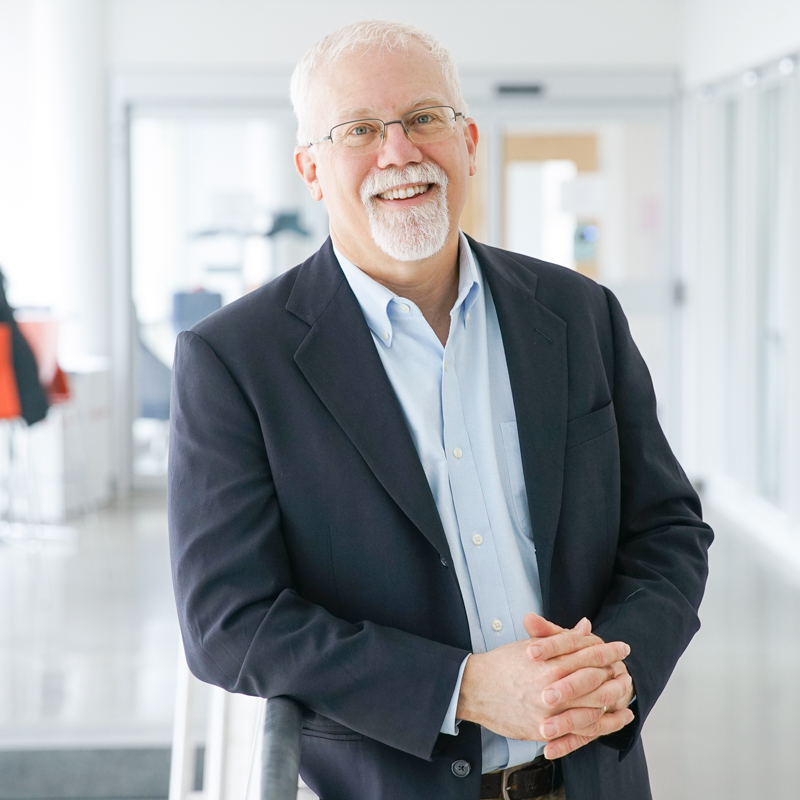
\includegraphics[width=\textwidth]{eppinger.jpg}
            \begin{center}
                Jeffrey Eppinger (1960)
            \end{center}
        \end{column}
    \end{columns}
\end{frame}

\begin{frame}[plain]
    \begin{center}
        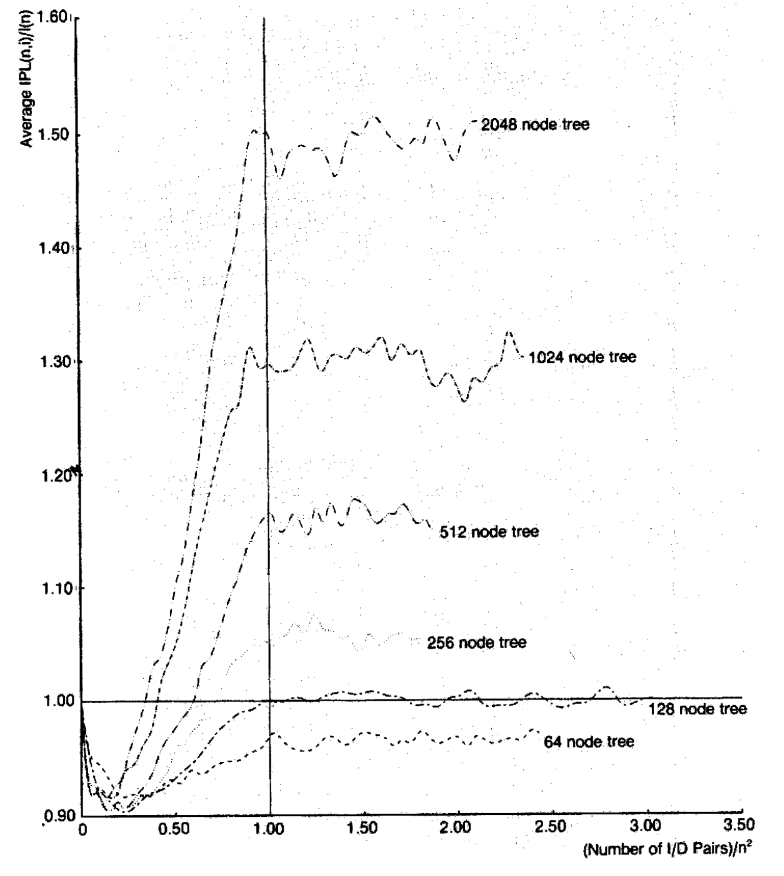
\includegraphics[width=\paperwidth,height=\paperheight,keepaspectratio]{plotEppinger.png}
    \end{center}
\end{frame}

\begin{frame}
    \footnotesize
    \begin{algorithmic}
        \Function{Symmetric delete}{$T$, $x$}
        \If{$T.val < x$}
        \State $T.right \gets$ \Call{Symmetric delete}{$T.right$, $x$}
        \ElsIf{$T.val > x$}
        \State $T.left \gets$ \Call{Symmetric delete}{$T.left$, $x$}
        \Else
        \If{$T.right = \text{null}$}
        \State \Return $T.left$
        \Else
        \If{\Call{flipCoin} $= Head$}
        \State $T.val \gets$ \Call{minValue}{$T.right$}
        \State $T.right \gets$ \Call{Symmetric delete}{$T.right$, $T.val$}
        \Else
        \State $T.val \gets$ \Call{maxValue}{$T.left$}
        \State $T.left \gets$ \Call{Symmetric delete}{$T.left$, $T.val$}
        \EndIf
        \EndIf
        \EndIf
        \State \Return $T$
        \EndFunction
    \end{algorithmic}
\end{frame}

\begin{frame}[plain]
    \begin{center}
        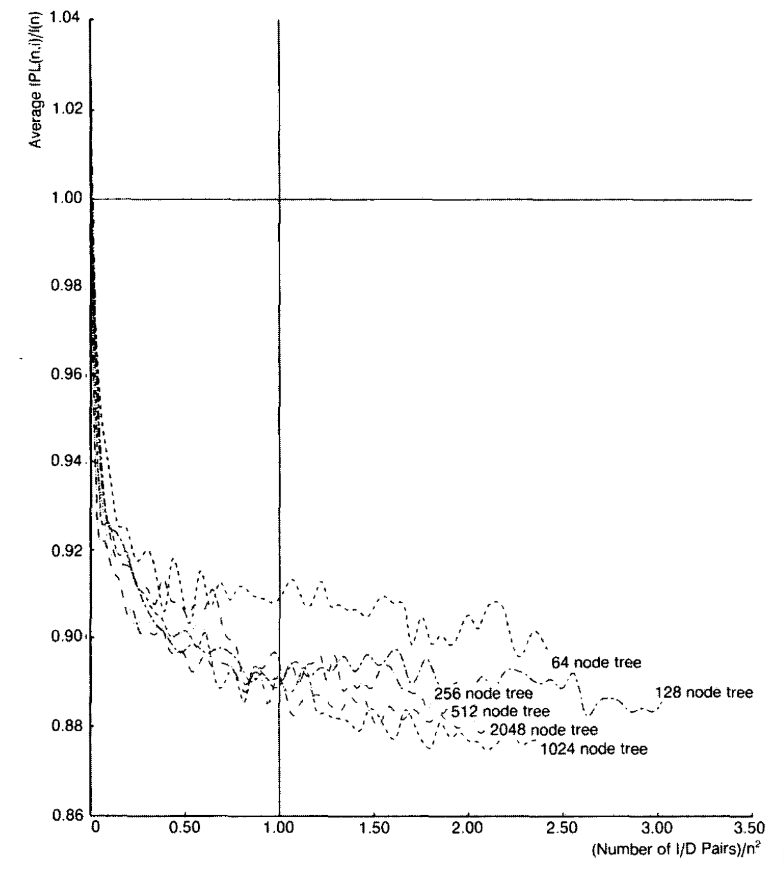
\includegraphics[width=\paperwidth,height=\paperheight,keepaspectratio]{plotEppingerSym.png}
    \end{center}
\end{frame}

\printbibliography
\frame{\titlepage}


\end{document}
